\documentclass{article}
\usepackage{graphicx, physics, enumitem, gensymb} % Required for inserting images
\usepackage[margin=1.4cm]{geometry}
\usepackage{tikz, float,cancel,xfrac}
\usepackage{upgreek}
\newcommand{\tund}[1]{_{\text{\tiny #1}}}
\usepackage{fixltx2e,graphicx}
\newcommand{\SE}{\mathcal{E}}
\usepackage[dvipsnames]{xcolor}
\newcommand{\SH}{\mathcal{H}}
\newcommand{\spi}[2]{S_{#1}^{#2}}
\newcommand{\SF}{\mathcal{F}}
\newcommand{\vk}{\vb{k}}
\newcommand{\sm}{\mathord{\scalebox{0.6}[1]{$-$}}}
\newcommand{\vkd}{\vb{k}'}
\newcommand{\vks}{\vb{k}\sigma}
\newcommand{\vkdsd}{\vb{k}\sigma}
\newcommand{\mkms}{\sm\vb{k},\sm\sigma}
\newcommand{\mkdmsd}{\sm\vb{k}',\sm\sigma'}
\usepackage{dsfont}
\newcommand{\cksd}{c^{\dagger}_{\vks}}
\newcommand{\ckdsd}{c_{\vkdsd}}
\newcommand{\cmkmsd}{c^{\dagger}_{\mkms}}
\newcommand{\cmkdmsd}{c_{\mkdmsd}}
\newcommand{\kup}{\vk\uparrow}
\newcommand{\kdown}{\sm\vk\downarrow}
\newcommand{\kdup}{\vk'\uparrow}
\newcommand{\kddown}{\sm\vk'\downarrow}
\newcommand{\cks}{c_{\vks}}
\newcommand{\Tc}{T\tund{c}^{\sm}}
\newcommand{\cd}{c^\dagger}
\newcommand{\ek}{\eta_{\vk}}
\newcommand{\gk}{\gamma_{\vk}}
\begin{document}
\hrule \vspace*{0.1cm}
\hrule
\begin{center}
    {\Large\bfseries Superconductivity}\par
    \vspace{0.35em}
    {\large\bfseries \textcolor{blue}{Notes}}\par
\end{center}
\hrule \vspace*{0.1cm}
\hrule
\vspace{0.5cm}
We assume that we understand the origin of the effective electron-electron interaction and what we have as the starting point is the reduced BCS Hamiltonian which is given by,
\begin{equation}
\SH = \sum\limits_{\vk, \sigma}\xi_{\vk}\cksd\cks + \sum\limits_{\vk, \vkd, \sigma}V_{\vk\vkd}\cksd\cmkmsd\cmkdmsd\ckdsd
\end{equation}
We consider only interactions from the pair $(\vk,\sigma)$ and $(-\vk, -\sigma)$ which are on the opposite sides of the Fermi surface, from which we get the Hamiltonian as,
\begin{equation}
    \SH = \sum\limits_{\vk, \sigma}\xi_{\vk}\cksd\cks + \sum\limits_{\vk, \vkd}V_{\vk\vkd}\cd_{\kup}\cd_{\kdown}c_{\kddown}c_{\kdup}
\end{equation}
Given this Hamiltonian, there are only are few things that can be done absolutely analytically. The simplest thing to impose on any such complicated system is the mean-field treatment, where we consider a slight fluctuation from the average quantity. In this case we consider the averages,
\begin{equation}
    b_{\vk} = \expval{c_{\kdown}c_{\kup}} \qquad  b_{\vk}^* = \expval{\cd_{\kup}\cd_{\kdown}}
\end{equation}
and then we consider the fluctuations,
\begin{align}
  \begin{split}
      c_{\kdown}c_{\kup} &=(c_{\kdown}c_{\kup} - b_{\vk}) + b_{\vk} \equiv  \delta b_{\vk}+b_{\vk}\\
    \cd_{\kup}\cd_{\kdown} &=( \cd_{\kup}\cd_{\kdown} - b_{\vk}^*) + b_{\vk}^* \equiv  \delta b_{\vk}^\dagger+b_{\vk}^*
  \end{split}
\end{align}
Using this, the interaction term of the reduced BCS Hamiltonian becomes,
\begin{align}
    V_{\vk\vkd}\qty(\delta b_{\vk}^\dagger+b_{\vk}^*)(\delta b_{\vk'}+b_{\vk'}) =  V_{\vk\vkd}\qty[\delta b_{\vk}^\dagger b_{\vk'} + b_{\vk}^*\delta b_{\vk'} + b_{\vk}^*b_{\vk'}]
\end{align}
where we had neglected the term which is second-order in fluctuations. Substituting this, the Hamiltonian becomes:
\begin{align}
   \begin{split}
     \SH &= \sum\limits_{\vk, \sigma}\xi_{\vk}\cksd\cks + \sum\limits_{\vk, \vkd}V_{\vk\vkd} \qty[b_{\vk}^*\qty(c_{\kddown}c_{\kdup}-b_{\vk}) +{b_{\vk}^*b_{\vk'}} + \qty(\cd_{\kup}\cd_{\kdown} - b_{\vk}^*)b_{{\vk}'}]\\
    &=\sum\limits_{\vk, \sigma}\xi_{\vk}\cksd\cks + \sum\limits_{\vk, \vkd}V_{\vk\vkd} \qty[b_{\vk}^*c_{\kddown}c_{\kdup} + b_{{\vk}'}\cd_{\kup}\cd_{\kdown} - b_{\vk}^*b_{{\vk}'}]
   \end{split}
\end{align}
We define the superconducting gap parameters,
\begin{equation}
    \Delta_{\vkd}^* = - \sum\limits_{\vk} V_{\vk\vkd}b_{\vk}^* \qquad\qquad \Delta_{\vk} = - \sum\limits_{\vkd} V_{\vk\vkd}b_{\vkd}
\end{equation}
Writing the Hamiltonian in terms of the gap parameters we get,
\begin{equation}
    \SH = \sum\limits_{\vk, \sigma}\xi_{\vk}\cksd\cks - \sum\limits_{\vk}\qty( \Delta_{\vk}^*c_{\kdown}c_{\kup} + \Delta_{\vk}c^\dagger_{\kup}c^\dagger_{\kdown} - b_{\vk}^*\Delta_{\vk})
\end{equation}
The first term in the interaction looks like a \textit{pair-annihilation} term, where the pair $(\vk,\uparrow)$ and $(-\vk,\downarrow)$ is destroyed while the second term looks like a \textit{pair-production} term, where the pair $(\vk,\uparrow)$ and $(-\vk,\downarrow)$ is created.\\[0.2cm]
\textbf{\large Change of Basis}\\[0.2cm]
Here we introduce two new spin-summed operators $\eta_{\vk}$ and $\gamma_{\vk}$ by the following transformation,
\begin{equation}
    \mqty(c_{\kup}\\ c_{\kdown}^\dagger) = \mqty(\cos\theta & -\sin\theta \\ \sin\theta & \cos\theta) \mqty(\eta_{\vk}\\ \gamma_{\vk})
\end{equation}
Substituting these definitions in the Hamiltonian we obtain,
\begin{align}
    \begin{split}
        \SH &= \sum\limits_{\vk, \sigma}\xi_{\vk}\cksd\cks - \sum\limits_{\vk}\Big[ \Delta_{\vk}^*\qty(\sin\theta \eta_{\vk}^\dagger +\cos\theta \gamma_{\vk}^\dagger )\qty(\cos\theta \eta_{\vk}-\sin\theta \gamma_{\vk})\\
        &\quad\hspace*{2cm}+\Delta_{\vk}\qty(\cos\theta \eta_{\vk}^\dagger -\sin\theta \gamma_{\vk}^\dagger)\qty(\sin\theta \eta_{\vk}+\cos\theta \gamma_{\vk}) - b_{\vk}^*\Delta_{\vk}\Big]
    \end{split}
\end{align}
The first sum can be broken down as,
\begin{equation}
   \sum\limits_{\vk} ( c_{\kup}^\dagger c_{\kup} + c_{\vk\downarrow}^\dagger c_{\vk\downarrow})\xi_{\vk} = \sum\limits_{\vk} ( c_{\kup}^\dagger c_{\kup}\xi_{\vk}) +\sum\limits_{\vk} (c_{\vk\downarrow}^\dagger c_{\vk\downarrow})\xi_{\vk}
\end{equation}
Since the second term is a sum over all $\vk$'s, we can make the replacement $\vk \leftrightarrow -\vk$ and noting that $\xi_{\vk} = \xi_{-\vk}$ we finally obtain,
\begin{equation}
     \sum\limits_{\vk} ( c_{\kup}^\dagger c_{\kup} + c_{\vk\downarrow}^\dagger c_{\vk\downarrow})\xi_{\vk} =  \sum\limits_{\vk} ( c_{\kup}^\dagger c_{\kup} + c_{\kdown}^\dagger c_{\kdown})\xi_{\vk}
\end{equation}
Let us now explicitly calculate this horrendous sum. We will denote $\cos$ with $c$ and $\sin$ with $s$ for brevity.
\begin{align}
    \begin{split}
        \SH =\sum\limits_{\vk} \Big[(c\ek^\dagger -s\gk^\dagger)(c\ek &-s\gk) + (s\ek +c\gk)(s\ek^\dagger +c\gk^\dagger)\Big]\xi_{\vk}-\ek^\dagger\ek (\Delta_{\vk}^*+\Delta_{\vk})(sc)\\
& -\gk^\dagger\gk (\Delta_{\vk}^*+\Delta_{\vk})(sc) +\ek^\dagger\gk (\Delta_{\vk}^*s^2-\Delta_{\vk}c^2) -\gk^\dagger\ek (\Delta_{\vk}^*c^2-\Delta_{\vk}s^2)+ b_{\vk}^*\Delta_{\vk}
    \end{split}
\end{align}
Expanding the first term we get some more lengthy things, 
\begin{align}
    \begin{split}
        \SH &=\sum\limits_{\vk} (\mathcolor{blue}{c^2\ek^\dagger\ek} - cs \ek^\dagger\gk - sc \gk^\dagger\ek +\mathcolor{red}{s^2 \gk^\dagger\gk})\xi_{\vk} +(\mathcolor{blue}{s^2\ek\ek^\dagger} +cs \ek\gk^\dagger + sc \gk\ek^\dagger+\mathcolor{red}{c^2\gk\gk^\dagger})\xi_{\vk}\\
        &-\ek^\dagger\ek (\Delta_{\vk}^*+\Delta_{\vk})(sc)-\gk^\dagger\gk (\Delta_{\vk}^*+\Delta_{\vk})(sc) +\ek^\dagger\gk (\Delta_{\vk}^*s^2-\Delta_{\vk}c^2) -\gk^\dagger\ek (\Delta_{\vk}^*c^2-\Delta_{\vk}s^2)+ b_{\vk}^*\Delta_{\vk}
    \end{split}
\end{align}
We now use the following things to somewhat simplify the crap that we have created,
$$\sin^2x + \cos^2x=1 \qquad \ek\ek^\dagger = 1- \ek^\dagger\ek \qquad \gk\gk^\dagger = 1- \gk^\dagger\gk\qquad \{\ek,\gk\}=\{\ek^\dagger,\gk^\dagger\}=\{\ek^\dagger,\gk\}=\{\ek,\gk^\dagger\}=0$$
Using the commutation relation and the trig identity, we can now group the terms in the Hamiltonian, 
\begin{align}
    \begin{split}
        \SH &= \sum\limits_{\vk} (\mathcolor{blue}{c^2\ek^\dagger\ek} - cs \ek^\dagger\gk - sc \gk^\dagger\ek +\mathcolor{red}{s^2 \gk^\dagger\gk})\xi_{\vk} +
        (\mathcolor{blue}{s^2 - s^2\ek^\dagger\ek} +cs \ek\gk^\dagger + sc \gk\ek^\dagger+\mathcolor{red}{c^2 - c^2\gk^\dagger\gk})\xi_{\vk}\\
        &\quad\qquad-\ek^\dagger\ek (\Delta_{\vk}^*+\Delta_{\vk})(sc)-\gk^\dagger\gk (\Delta_{\vk}^*+\Delta_{\vk})(sc) +\ek^\dagger\gk (\Delta_{\vk}^*s^2-\Delta_{\vk}c^2) -\gk^\dagger\ek (\Delta_{\vk}^*c^2-\Delta_{\vk}s^2) + b_{\vk}^*\Delta_{\vk}\\
        &=\sum\limits_{\vk} \mathcolor{OliveGreen}{\ek^\dagger \ek \qty[(c^2-s^2)\xi_{\vk} - (sc)(\Delta_{\vk}^* + \Delta_{\vk})]} + \mathcolor{magenta}{\xi_{\vk}({s^2+c^2}) + \Delta_{\vk}b_{\vk}^*}+\mathcolor{OliveGreen}{\gk^\dagger\gk \qty[(s^2-c^2)\xi_{\vk} + (sc)(\Delta_{\vk}^* + \Delta_{\vk})]} \\
        &\quad\qquad+ \gk^\dagger\ek \qty[-2sc\xi_{\vk} -(\Delta_{\vk}^*c^2-\Delta_{\vk}s^2)] + \ek^\dagger\gk\qty[-2sc\xi_{\vk} + (\Delta_{\vk}^* s^2 - \Delta_{\vk}c^2)]
    \end{split} 
\end{align}
The \textcolor{OliveGreen}{green} terms are the direct quadratic terms while the \textcolor{magenta}{magenta} term is a constant energy shift (operator independent term). The black terms are the cross-terms. We want to get rid of these cross-terms (by equating their coefficients to zero) and for that we can choose a particular value of $\theta$. Let us now assume that the complex phase fluctuations are negligible, such that $\Delta_{\vk} = \Delta_{\vk}^*$ from which the coefficient of one of the cross terms become,
\begin{equation}
    -2sc\xi_{\vk} - \Delta_{\vk}(c^2-s^2) = 0 \implies -\xi_{\vk} \sin 2\theta  - \Delta_{\vk} \cos 2\theta =0 \implies \tan 2\theta = -\frac{\Delta_{\vk}}{\xi_{\vk}}
\end{equation}
Now, to obtain $\tan\theta$ we can first define $E_{\vk} = \sqrt{\xi_{\vk}^2+\Delta_{\vk}^2}$ and then use the identity,
$$\tan\theta = \frac{-1 \pm \sqrt{1+\tan^2 2\theta}}{\tan 2\theta} = \frac{-1 \pm \frac{ \sqrt{\xi_{\vk}^2+\Delta_{\vk}^2}}{\xi_{\vk}}}{\Delta_{\vk}}\times \xi_{\vk} = \frac{E_{\vk}-\xi_{\vk}}{\Delta_{\vk}}$$
from which we can find the values,
\begin{align}
    \sin^2\theta &= \frac{(E_{\vk}-\xi_{\vk})^2}{(E_{\vk}-\xi_{\vk})^2+\Delta_{\vk}^2} =\frac{(E_{\vk}-\xi_{\vk})}{(E_{\vk}-\xi_{\vk})+\frac{E_{\vk}^2-\xi_{\vk}^2}{(E_{\vk}-\xi_{\vk})}} = \frac{(E_{\vk}-\xi_{\vk})}{(E_{\vk}-\xi_{\vk})+E_{\vk}+\xi_{\vk}} =  \frac{1}{2}\qty(1 - \frac{\xi_{\vk}}{E_{\vk}})\equiv v_{\vk}^2\\
    \cos^2\theta &= \frac{\Delta_{\vk}^2}{(E_{\vk}-\xi_{\vk})^2+\Delta_{\vk}^2} =\frac{(E_{\vk}^2-\xi_{\vk}^2)}{(E_{\vk}-\xi_{\vk})^2+E_{\vk}^2-\xi_{\vk}^2} = \frac{E_{\vk}+\xi_{\vk}}{(E_{\vk}-\xi_{\vk}) +E_{\vk}+\xi_{\vk}} = \frac{1}{2}\qty(1 + \frac{\xi_{\vk}}{E_{\vk}})\equiv u_{\vk}^2
\end{align}
These $u_{\vk}^2$ and $v_{\vk}^2$ are called \textit{coherence factors}. Using these we can write, $(\cos^2\theta-\sin^2\theta) = \sfrac{\xi_{\vk}}{E_{\vk}}$ and $\sin\theta\cos\theta = -\sfrac{\abs{\Delta_{\vk}}}{2E_{\vk}}$. With the cross-terms gone and with the definitions of these coherence factors, we can write the simplified Hamiltonian as,
\begin{align}
     \begin{split}
      \SH &=\sum\limits_{\vk} {\ek^\dagger \ek \qty[\frac{\xi_{\vk}^2}{E_{\vk}} + \frac{\abs{\Delta_{\vk}}}{2E_{\vk}}(2 \Delta_{\vk})]} +{\xi_{\vk} + \Delta_{\vk}b_{\vk}^*}+{\gk^\dagger\gk \qty[-\frac{\xi_{\vk}^2}{E_{\vk}}  - \frac{\abs{\Delta_{\vk}}}{2E_{\vk}}(2\Delta_{\vk})]}\\
      &=\sum\limits_{\vk}\qty(\ek^\dagger \ek - \gk^\dagger \gk)\qty(\frac{\xi_{\vk}^2+ \Delta_{\vk}^2}{E_{\vk}}) + \qty({\xi_{\vk} + \Delta_{\vk}b_{\vk}^*})\\
      &=\sum\limits_{\vk}\qty({\xi_{\vk} + \Delta_{\vk}b_{\vk}^*}) + \sum\limits_{\vk} \qty(\ek^\dagger \ek - \gk^\dagger \gk)E_{\vk} \equiv \SH\tund{0} +\widetilde{\SH}
    \end{split}
\end{align}
The first sum denotes a operator independent part of the Hamiltonian, $\SH\tund{0}$ and hence it just causes a shift in the energy and contains no \textit{fermionic} degrees of freedom. The second sum resembles the free-fermionic quadratic Hamiltonian $\widetilde{\SH}$, however, the energies need to be looked carefully. For $\ek$ we have the quasiparticle excitation energy $E\to E_{\vk}$ while for $\gk$ we have the energy $E\to -E_{\vk}$. Thus these are two ``species'' of fermions described by the operators $\ek$ and $\gk$.\\[0.2cm]
Also note that from the definition, if $\xi_{\vk} =0$ (which defines the \textit{Fermi surface}), we have $E_{\vk} = \Delta_{\vk}$. Thus, there is a gap in the spectrum and thus $\Delta_{\vk}$ is called the \textit{superconducting gap parameter}. \\[0.3cm]
\textbf{\large Grand Canonical Description}\\[0.2cm]
Let us find the grand partition function,
\begin{equation}
    \Xi \equiv \tr\qty(e^{-\beta \SH}) = \tr\qty(e^{-\beta (\SH\tund{0}+\widetilde{\SH})}) = \tr\qty(e^{-\beta \SH\tund{0}}e^{-\beta \widetilde{\SH}}) = e^{-\beta \SE\tund{0}}\tr\qty(e^{-\beta \widetilde{\SH}})
\end{equation}
where we used the fact that $\SH\tund{0}\propto\mathds{1}$ and hence it commutes with everything. Different quasiparticle modes are independent and hence the exponential factorises.
\begin{equation}
    \begin{split}
        \Xi = e^{-\beta \SE\tund{0}}\prod\limits_{\vk}\tr\qty[e^{-\beta E_{\vk}\qty(\ek^\dagger\ek - \gk^\dagger\gk)}]
    \end{split}
\end{equation}
The eigenvalues of $\hat{n}_{\eta} \equiv \ek^\dagger\ek$ and $\hat{n}_{\gamma} \equiv\gk^\dagger\gk$ can be $\{0,1\}$ since these are kinda like fermionic number operators and hence we get four possibilities, for $\mathcolor{red}{n_{\eta}} - \mathcolor{blue}{n_{\gamma}}$ after taking the trace.
\begin{equation}
   \begin{split}
     \Xi &=  e^{-\beta \SE\tund{0}}\prod\limits_{\vk}\qty[\underbrace{1}_{\mathcolor{red}{0} - \mathcolor{blue}{0}} + \underbrace{e^{-\beta E_{\vk}}}_{{\mathcolor{red}{1} - \mathcolor{blue}{0}}} + \underbrace{e^{\beta E_{\vk}}}_{\mathcolor{red}{0} - \mathcolor{blue}{1}}+\underbrace{1}_{\mathcolor{red}{1} - \mathcolor{blue}{1}}]\\
    &= e^{-\beta \SE\tund{0}}\prod\limits_{\vk}\qty(1+e^{\beta E_{\vk}})(1+e^{-\beta E_{\vk}})\equiv e^{-\beta \SF}
   \end{split}
\end{equation}
Then the free energy $\SF$ can be written as, 
\begin{equation}
    \SF = \SE\tund{0} - \frac{1}{\beta}\sum\limits_{\vk}\ln\qty[(1+e^{\beta E_{\vk}})(1+e^{-\beta E_{\vk}})]
\end{equation}
Suppose now we want to see what happens at the zero temperature limit, when $T\to 0$. Then note that, 
\begin{align}
    1 + e^{ \pm \beta E_{\vk}} &= e^{\pm\beta E_{\vk}}\Theta(\pm E_{\vk}) + (1-\Theta(\pm E_{\vk})) \implies \frac{1}{\beta}\ln\qty(1 + e^{ \pm \beta E_{\vk}}) = \pm E_{\vk}\Theta(\pm E_{\vk})
\end{align}
where $\Theta(x)$ is the Heaviside step function. Then the free energy becomes,
\begin{align}
   \begin{split}
     \SF &= \SE\tund{0} +\sum\limits_{\vk} E_{\vk}\Theta(-E_{\vk})-E_{\vk}\Theta(E_{\vk})\\
    &=\SE\tund{0} +\sum\limits_{\vk} E_{\vk}(1 - \Theta(E_{\vk}))-E_{\vk}\Theta(E_{\vk})\\
    &=\SE\tund{0} +\sum\limits_{\vk} E_{\vk}(1 - 2\Theta(E_{\vk})) = \sum\limits_{\vk}(\xi_{\vk} +\Delta_{\vk}b_{\vk}^*) -\sum\limits_{\vk} E_{\vk}
   \end{split}
\end{align}
where we used that $E_{\vk}>0$ always so $\Theta(E_{\vk})=1$ for all $\vk$'s. Anyways, this was like a digression. We now want to minimize the free energy using $\Delta_{\vk}$ as a variational parameter. 
\begin{align}
    \begin{split}
        \pdv{\SF}{\Delta_{\vk}} &= b_{\vk}^* -\frac{1}{\cancel{\beta}}\qty[\frac{-\cancel{\beta} e^{-{\beta} E_{\vk}}}{1+e^{-\beta E_{\vk}}} +\frac{\cancel{\beta} e^{\beta E_{\vk}}}{1+e^{\beta E_{\vk}}}]\times \pdv{E_{\vk}}{\Delta_{\vk}}\\
        &=b_{\vk}^* +\pdv{E_{\vk}}{\Delta_{\vk}} \qty[\frac{e^{-{\beta} E_{\vk}}}{1+e^{-\beta E_{\vk}}} -\frac{ e^{\beta E_{\vk}}}{1+e^{\beta E_{\vk}}}]  = 0
    \end{split}
\end{align}
Now, note that using $E_{\vk} = \sqrt{\xi_{\vk}^2+\Delta_{\vk}^2}$, we get $\sfrac{\partial E_{\vk}}{\partial \Delta_{\vk}} =\sfrac{ E_{\vk}}{\Delta_{\vk}} $ using which which we get,
\begin{align}
    \begin{split}
        b_{\vk}^* = -\frac{\Delta_{\vk}}{E_{\vk}}\qty[\frac{e^{-\beta E_{\vk}} + 1 - e^{\beta E_{\vk}}-1}{1 + e^{\beta E_{\vk}} + e^{-\beta E_{\vk} }+1}] = \frac{\Delta_{\vk}}{E_{\vk}}\qty[\frac{2\sinh(\beta E_{\vk})}{2(1+\cosh(\beta E_{\vk}))}] =\frac{\Delta_{\vk}}{E_{\vk}} \qty[\frac{2\sinh(\beta E_{\vk}/2)\cosh(\beta E_{\vk}/2)}{2 \cosh^2(\beta E_{\vk}/2)}]
    \end{split}
\end{align}
\textcolor{red}{check the missing factor of $2$!!}\\
The minimization gives us, 
\begin{equation}
    b_{\vk}^* = \Delta_{\vk}\qty[\frac{\tanh(\beta E_{\vk}/2)}{2E_{\vk}}] \equiv \Delta_{\vk}\upchi_{\vk}
\end{equation}
where $\xi_{\vk}$ is called the \textit{piar susceptibility} and denotes the ability to form Cooper pair. Then, the superconducting gap becomes, 
\begin{equation}
    \Delta_{\vk} = - \sum\limits_{\vkd}V_{\vk \vkd} b_{\vkd} = - \sum\limits_{\vkd}V_{\vk \vkd}\qty[\frac{\tanh(\beta E_{\vkd}/2)}{2E_{\vkd}}]\Delta_{\vkd}
    \label{eqn:gapeq}
\end{equation}
This is a self-consistent equation since both LHS and RHS consists of $\Delta_{\vk}$. This is the famous \textit{BCS gap equation} and it applies to any superconductor, irrespective of the origin of the effective electron-electron attraction (though we derived this using phononic degrees of freedom of the lattice).\\[0.2cm]
\textbf{\underline{s-wave superconductor}}:\\[0.2cm]
Now, let us assume that the potential is constant in a thin shell around the Fermi surface of thickness $\sim \hbar \omega\tund{D}$ where $\omega\tund{D}$ is the Debye frequency cutoff, and zero otherwise, 
\begin{equation}
    V_{\vk\vkd} = \begin{cases}
        -V & \abs{\xi_{\vkd}}, \abs{\xi_{\vk}}\leq \hbar \omega\tund{D}\\
        0 & \text{else}
    \end{cases}
\end{equation}
Then the simplified gap equation becomes,
\begin{equation}
    \frac{\Delta_{\vk}}{V} = \sum\limits_{\substack{\vk \in \text{thin}\\\text{\ \ \ \ shell}}} \frac{\tanh(\beta E_{\vkd}/2)}{2E_{\vkd}}\Delta_{\vkd}
\end{equation}
Note that, the RHS is independent of $\vk$ thus, $\Delta_{\vk}$ is not a function of $\vk$ and hence, is a constant, say $\Delta\tund{0}$. Now, note that $\Delta\tund{0}=0$ is a trivial solution, satisfying the above equation. If $\Delta\tund{0}\neq 0$ we can cancel it from both sides giving us, 
\begin{equation}
    \frac{1}{V} = \sum\limits_{\substack{\vk \in \text{thin}\\\text{\ \ \ \ shell}}} \frac{\tanh(\beta E_{\vkd}/2)}{2E_{\vkd}}
\end{equation}
Let us now examine what happens in the limit of zero temperature, that is, $\beta\to \infty$.\\[0.2cm]
\textbf{\underline{Zero temperature limit}:}\\[0.2cm]
In this case, $\tanh(x)\to 1$ since $x\sim \beta$ is very large. We now change the finite sum over $\vkd$ to an integral near the Fermi surface where the density of states is approximately constant$\sim \mathcal{N}(\SE\tund{F})$,
\begin{equation}
    \frac{1}{V} = \int\limits_{-\hbar \omega\tund{D}}^{\hbar \omega\tund{D}}\mathcal{N}({\xi}) \dd \xi\ \frac{1}{2\sqrt{\Delta^2 + \xi^2}} \simeq \frac{1}{2}\mathcal{N}(\SE\tund{F})  \int\limits_{-\hbar \omega\tund{D}}^{\hbar \omega\tund{D}}\ \frac{\dd \xi}{\sqrt{\Delta^2 + \xi^2}} = \mathcal{N}(\SE\tund{F}) \int\limits_{0}^{\hbar \omega\tund{D}}\ \frac{\dd \xi}{\sqrt{\Delta^2 + \xi^2}}
\end{equation}
Let us define $\xi = \Delta x$ and $\lambda = V \mathcal{N}(\SE\tund{F})$. Then, the integral becomes,
\begin{equation}
    \frac{1}{\lambda} = \int\limits_{0}^{\hbar \omega\tund{D}/\Delta}\frac{\dd x}{\sqrt{1+x^2}}= \sinh^{-1}\qty(\frac{\hbar \omega\tund{D}}{\Delta})
\end{equation}
If $\lambda\ll 1$, the RHS becomes very large which happens in the limit $\hbar \omega\tund{D} \gg 1$. In that case, note that, 
\begin{equation}
    \sinh(x) = \frac{e^x-e^{-x}}{2}\xrightarrow{x\gg 1} \frac{e^x}{2}\implies \sinh^{-1}(x) \approx \ln(2x)\qquad \text{for large $x$}
\end{equation}
Using this approxmation we obtain,
\begin{equation}
    \frac{1}{\lambda} \approx \ln\qty(\frac{2\hbar \omega\tund{D}}{\Delta}) \implies \boxed{\Delta\tund{0} = 2\hbar \omega\tund{D} e^{-1/\lambda}}\longrightarrow \text{finite}
\end{equation}
\textbf{\underline{Infinite temperature limit}:}\\[0.2cm]
In this case, $\beta\to 0$ and hence the gap equation becomes $\Delta\tund{0} = 0$. Thus, in the infinite temperature limit, $\Delta\tund{0}=0$ is the only solution. 

This fact tells us that there is a transition temperature $T\tund{c}$ where the behaviour of the gap parameter changes from being finite to zero. Let us consider the case when $T\to \Tc$ such that $\Delta\to 0$, which gives us, $E_{\vk} = \xi_{\vk}$. Then changing the sum to integral gives us, 
\begin{equation}
    \frac{1}{\lambda} = \int\limits_{0}^{\hbar \omega\tund{D}}\dd\xi\ \frac{\tanh(\beta\tund{c} \xi)}{\xi}\quad \xrightarrow[\text{by parts}]{\text{integration}}\quad -\int\limits_{0}^{\beta\tund{c} \hbar \omega\tund{D}/2} \dd x \ \frac{\ln x}{\cosh^2 x} + \tanh\qty(\beta\omega\tund{D}/2)\ln\qty(\beta\omega\tund{D}/2)
\end{equation}
\begin{figure}[h]
    \centering
    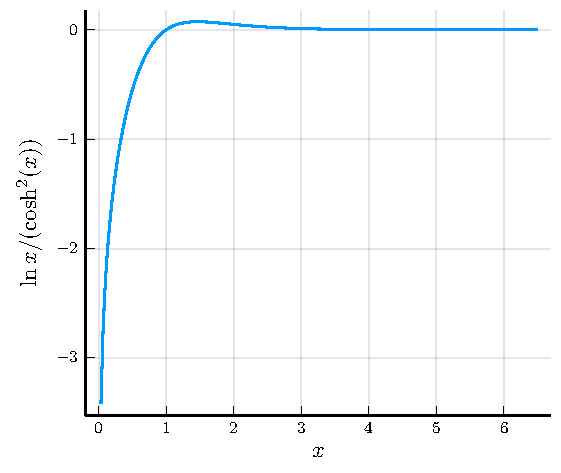
\includegraphics[width=0.45\textwidth]{bcs.pdf}
\end{figure}
Now, look at the plot of $\frac{\ln x}{\cosh^2 x}$ above, which has most of the contributions near $x\to 0$ and falls pretty fast to zero as we increase $x$. Hence in the above integral, we can safely extend the upper limit upto $\infty$, with negligible contributions. The integral gives us $\upgamma - \ln\qty(\pi/4)$ where $\upgamma\approx 0.577215\ldots$ is the \textit{Euler-Mascheroni constant}. Also, taking the argument $\beta\omega\tund{D}$ to be large, (giving us $\tanh\qty(\beta\omega\tund{D}/2)\to 1$), we finally obtain: 
\begin{equation}
    \frac{1}{\lambda} = \upgamma - \ln\qty(\pi/4) + \ln\qty(\beta\omega\tund{D}/2)\implies \frac{1}{\lambda} = \ln\qty[\frac{\beta\omega\tund{D}e^{\upgamma}}{\pi/2}] = \ln \qty[\frac{2\beta\tund{c}\omega\tund{D}}{\pi}e^{\upgamma}]\implies \boxed{k\tund{B}T\tund{c} = \frac{2e^{\upgamma}}{\pi}\omega\tund{D}e^{-1/\lambda}}
\end{equation}
which gives us the expression of the transition temperature. Note that both the results at zero temperature and at the transition temperature has an $e^{-1/\lambda}$ term which has an essential singularity as $\lambda\to 0$ which is the perturbative regime. Hence, these results cannot be obtained perturbatively. Moreover, $\lambda$ being a microscopic parameter of the particular model, cannot be determined experimentally. However, we can divide both the results to obtain,
\begin{equation}
    \frac{2\Delta(T=0)}{k\tund{B}T\tund{c}} = \frac{2\pi}{e^{\upgamma}} \approx 3.52 \ \longrightarrow\text{ universal constant}
\end{equation}
\textbf{\underline{Generalized Gap Equation}:}\\[0.2cm]
We now forego the origin of attraction completely and focus only on the fact that the Cooper pairs are already formed. The electron movies in a crystal which has some underlying \textit{symmetries}. These symmetries must be reflected in any physical quantity that we consider and should be explainable in a complete set of functions, say $\{g_\beta(\vk)\}$ reflecting that symmetry. In that, we assume that the interaction potential is factorizable, that is,
\begin{equation}
    V_{\vk\vkd} = \sum\limits_{\beta} V_{\beta}\ g_\beta(\vk)g_\beta(\vkd)
\end{equation}
where $V_{\beta}$ denotes the strength of the interaction in the $\beta\sm$channel. We then substitute this expression in the gap equation Eq. \eqref{eqn:gapeq},
\begin{equation}
    \Delta_{\vk} = -\sum\limits_{\vkd,\beta} V_{\beta}\ g_\beta(\vk)g_\beta(\vkd)\Delta_{\vkd}\upchi_{\vkd} =-\sum\limits_{\beta} V_{\beta}\ g_\beta(\vk) \underbrace{\sum\limits_{\vkd} g_\beta(\vkd)\Delta_{\vkd}\upchi_{\vkd}}_{-\sfrac{\Delta_{\beta}}{V_{\beta}}}\equiv \sum\limits_{\beta}\Delta_{\beta}g_{\beta}(\vk)
\end{equation}
Thus, we see that the gap parameter is also expandable in the function $\{g_{\beta}\}$ with coefficients $\{\Delta_{\beta}\}$ which depend on the temperature. From our definition above we have,
\begin{align}
    \begin{split}
        \Delta_{\beta} &= -V_\beta\sum\limits_{\vkd}g_\beta(\vkd)\upchi_{\vkd}\mathcolor{red}{\Delta_{\vkd}}= -V_\beta\sum\limits_{\vkd,\mathcolor{red}{\alpha}}g_\beta(\vkd)\upchi_{\vkd}\mathcolor{red}{g_{\alpha}(\vkd)\Delta_{\alpha}}\implies \Delta_{\beta}\equiv \sum\limits_{\alpha}\mathcal{M}_{\beta\alpha}\Delta_{\alpha}
    \end{split}
\end{align}
where the matrix element, $\mathcal{M}_{\beta\alpha} := -V_\beta\sum\limits_{\vkd} g_{\alpha}(\vkd)g_{\beta}(\vk)\upchi_{\vkd}$. Let us try to see this in an example, which we consider it to be a simplified version of the \textbf{t-J model}, given by the Hamiltonian,
\begin{equation}
    \SH = -t \sum\limits_{\expval{ij}, \sigma} c_{i\sigma}^\dagger c_{j\sigma} + c_{j\sigma}^\dagger c_{i\sigma} + J\sum\limits_{\expval{ij}} \qty(\vb{S}_{i}\cdot \vb{S}_j - \frac{1}{4}n_{i}n_{j} )
\end{equation}
where $n_i$ is the spin-resolved number operator given by $n_i := n_{i\uparrow} + n_{i\downarrow}$. First let us simplify the above term,
\begin{align}
    \vb{S}_{i}\cdot \vb{S}_j =\mathcolor{red}{ \spi{i}{x}\spi{j}{x}+\spi{i}{y}\spi{j}{y}}+\spi{i}{z}\spi{j}{z}
\end{align}
We also define the spin raising and lowering operators, 
\begin{align}
    \spi{i}{\pm}:= \spi{i}{x}\pm \spi{i}{y} \implies \spi{i}{x}= \frac{1}{2}\qty(\spi{i}{+} + \spi{i}{-}) \qquad  \spi{i}{y}= \frac{1}{2i}\qty(\spi{i}{+} - \spi{i}{-})
\end{align}
Using this, the red terms become, 
\begin{align}
   \begin{split}
     \frac{1}{4}\qty(\spi{i}{+}+\spi{i}{-})\qty(\spi{j}{+}+\spi{j}{-})- \frac{1}{4}\qty(\spi{i}{+}-\spi{i}{-})\qty(\spi{j}{+}-\spi{j}{-}) &= \frac{1}{4}\qty[\cancel{\spi{i}{+}\spi{j}{+}}+\spi{i}{+}\spi{j}{-}+\spi{i}{-}\spi{j}{+}+\cancel{\spi{i}{-}\spi{j}{-}} - \cancel{\spi{i}{+}\spi{j}{+}} +\spi{i}{+}\spi{j}{-}+\spi{i}{-}\spi{j}{+} -\cancel{\spi{i}{-}\spi{j}{-}}]\\
    &=\frac{1}{2}\qty(\spi{i}{+}\spi{j}{-}+\spi{i}{-}\spi{j}{+})
   \end{split}
\end{align}
Then the second term in the Hamiltonian becomes, 
\begin{equation}
    \qty[\frac{1}{2}\qty(\spi{i}{+}\spi{j}{-}+\spi{i}{-}\spi{j}{+}) +\spi{i}{z}\spi{j}{z}]  - \frac{1}{4}n_in_j
\end{equation}
Now, note that we can write the spin operators in a second-quantized manner, 
\begin{equation}
    \spi{i}{+} = c_{i\uparrow}^{\dagger}c_{i\downarrow}\qquad \spi{i}{-} = c_{i\downarrow}^{\dagger}c_{i\uparrow}\qquad \spi{i}{z} = \frac{1}{2}(n_{i\uparrow}-n_{i\downarrow})
\end{equation}
using which gives us a terrible looking expression,
\begin{align}
    &\frac{1}{2}\qty[c_{i\uparrow}^{\dagger}c_{i\downarrow}c_{j\downarrow}^{\dagger}c_{j\uparrow}  +c_{i\downarrow}^{\dagger}c_{i\uparrow} c_{j\uparrow}^{\dagger}c_{j\downarrow}] + \frac{1}{4}\qty(n_{i\uparrow}-n_{i\downarrow})\qty(n_{j\uparrow}-n_{j\downarrow}) -\frac{1}{4}\qty(n_{i\uparrow}+n_{i\downarrow})\qty(n_{j\uparrow}+n_{j\downarrow})\\[0.1cm]
    =&\frac{1}{2}\qty[c_{i\uparrow}^{\dagger}c_{i\downarrow}c_{j\downarrow}^{\dagger}c_{j\uparrow}  +c_{i\downarrow}^{\dagger}c_{i\uparrow} c_{j\uparrow}^{\dagger}c_{j\downarrow} - \qty(n_{i\uparrow}n_{j\downarrow} + n_{i\downarrow}n_{j\uparrow})]
\end{align}
Then we perform a Fourier transform of these creation and annihilation operators (which I am not going to do for obvious reasons), the interaction term in Fourier space becomes,
\begin{equation}
    V_{\vk\vkd} = \frac{J}{4}\qty(\gk\gamma_{\vkd} + \ek\eta_{\vkd}) + 2J\qty(\sin k\tund{x}\sin k'\tund{x}+\sin k\tund{y}\sin k'\tund{y})
\end{equation}
where $\ek = 2(\cos k\tund{x} - \cos k\tund{y})$ and $\gk = 2(\cos k\tund{x} + \cos k\tund{y})$. This is a factorizable interaction term that we had formalized earlier. We can now use this to find a generalized gap equation, where the gap parameter is not constant but depends on $\vk$.\\[0.3cm]
While considering the Cooper pair, we focussed on two electrons on the opposite side of the Fermi surface, with momenta and spin: $(\vk, \uparrow)$ and $(-\vk, \downarrow)$. Thus, the wavefunction is formed of an orbital part and a spin part, 
\begin{equation}
    \mathrm{Cooper\ \ pair}\ \rightarrow\  \mathrm{orbital}\otimes\mathrm{spin}
\end{equation}
The complete two electron wavefunction should be anti-symmetric under electronic exchanges. Now consider two cases,\\[0.2cm]
\textbf{\underline{Singlet pairing}:}\\[0.2cm]
$$\ket{S=0} = \frac{1}{\sqrt{2}}\qty(\ket{\uparrow\downarrow} - \ket{\downarrow \uparrow}) $$
Note that the singlet state is anti-symmetric under the exchange of the up and the down spins, hence the orbital part should be \textit{symmetric} under exchange of the electron,
\begin{equation}
    \Psi\tund{orb}(1,2) = + \Psi\tund{orb}(2,1)
\end{equation}
\textbf{\underline{Triplet pairing}:}\\[0.2cm]
Consider any of the triplet states,
$$\ket{\uparrow\uparrow}\qquad\frac{\ket{\uparrow\downarrow} + \ket{\downarrow\uparrow}}{\sqrt{2}}\qquad\ket{\downarrow\downarrow}$$
Under any of the electron exchanges, these remain unchanged, hence the orbital part should be \textit{anti-symmetric} in this case. 
\begin{equation}
    \Psi\tund{orb}(1,2) = - \Psi\tund{orb}(2,1)
\end{equation}
In general, depending on the spin, the orbital part can be written as, 
\begin{align}
\begin{array}{cc}
\Psi_{\rm orb}(\vb r)=(-1)^l\Psi_{\rm orb}(-\vb r)
&
\begin{array}{l}
\circ\ \text{singlet} \to l\text{ even}: \quad
\overset{s}{0},\overset{d}{2},\overset{g}{4},\ldots \\[0.3em]
\circ\ \text{triplet} \to l\text{ odd}: \quad
\overset{p}{1},\overset{f}{3},\overset{h}{5},\ldots
\end{array}
\end{array}
\end{align}
Consider the interaction that we found out for the t-J model. Since $\sin(k_i)$ is odd under the exchange of $\vk$, it belongs to the odd parity sector. Then for considering the singlet case, we can safely drop the sin terms, giving us,
\begin{equation}
    V_{\vk\vkd}^{(s)} = \frac{J}{4}\qty(\gk\gamma_{\vkd}+\ek\eta_{\vkd})
\end{equation}
where the superscript $(s)$ stands for singlet. Now, consider a $90\degree$ rotation denoted by $\mathrm{R}$, of $\vk$ which changes $(k\tund{x},k\tund{y})\overset{\mathrm{R}}{\mapsto} (-k\tund{y}, k\tund{x})$. This rotation is a symmetry for the \textit{square lattice} and we note that $\gamma_{R\vk} = \cos(-k\tund{y}) + \cos k\tund{x} = \gk $ is invariant. This is called the \textit{extended s-wave}. Also, note that $\eta_{R\vk} = \cos(-k\tund{y}) - \cos(k\tund{x}) = -\ek$ which is called the \textit{d-wave}.  \\[0.3cm]
Now, let us derive the self-consistency equations for the t-J model. For that, let us consider the $T\to 0$ case where $\tanh(\beta E_{\vk})\to 1$ and then the gap equation becomes,
\begin{equation}
    \Delta_{\vk} = \frac{J}{4N} \sum\limits_{\vb{q}}\qty(\gk \gamma_{\vb{q}} +\ek \eta_{\vb{q}} ) \frac{\Delta_{\vb{q}}}{2E_{\vb{q}}}
\end{equation}
\end{document}

